\documentclass{article}
\usepackage{tikz}

\begin{document}

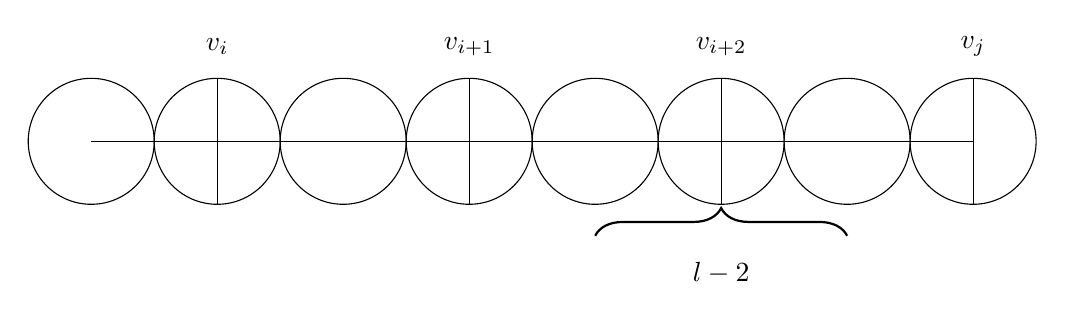
\begin{tikzpicture}[scale=0.8]
    % Draw circles
    \foreach \x in {0,...,7} {
        \draw (2*\x, 0) circle (1);
    }
    
    % Draw horizontal lines
    \draw (0, 0) -- (14, 0);
    \draw (2, -1) -- (2, 1);
    \draw (6, -1) -- (6, 1);
    \draw (10, -1) -- (10, 1);
    \draw (14, -1) -- (14, 1);
    
    % Label nodes
    \node at (2, 1.5) {$v_i$};
    \node at (6, 1.5) {$v_{i+1}$};
    \node at (10, 1.5) {$v_{i+2}$};
    \node at (14, 1.5) {$v_j$};
    
    % Dotted line
    \draw[dotted] (8, 0) -- (12, 0);
    
    % Label for l-2
    \draw[decorate, decoration={brace, amplitude=10pt}, thick] (8, -1.5) -- node[below=6pt] {$l-2$} (12, -1.5);
\end{tikzpicture}

\end{document}